\documentclass[12pt]{article}
\usepackage{url,graphicx,tabularx,array}
\usepackage[margin=1in]{geometry}
\setlength{\parskip}{1ex} %--skip lines between paragraphs
\setlength{\parindent}{0pt} %--don't indent paragraphs

\usepackage{algorithmic}
\usepackage{algorithm}
\usepackage{ amssymb }
\usepackage{ latexsym }
\usepackage{ amsmath }
\usepackage{ amsthm }
%-- Commands for header
\renewcommand{\title}[1]{\textbf{#1}\\}
\renewcommand{\line}{\begin{tabularx}{\textwidth}{X>{\raggedleft}X}\hline\\\end{tabularx}\\[-0.5cm]}
\newcommand{\leftright}[2]{\begin{tabularx}{\textwidth}{X>{\raggedleft}X}#1%
& #2\\\end{tabularx}\\[-0.5cm]}

\newtheorem{defn}{Definition}[section]
\newtheorem{conjecture}{conjecture}[section]
\newtheorem{lemma}{Lemma}[section]
\newtheorem{corollary}{Corollary}[section]
\newtheorem{question}{Question}[section]
\newtheorem{proposition}{Proposition}[section]


%\linespread{2} %-- Uncomment for Double Space
\begin{document}

\title{Homework 5: CMPS 242}
\line
\leftright{\today}{Bryan Matsuo (bmatsuo@soe.ucsc.edu) \& John St. John (jstjohn@soe.ucsc.edu)} %-- left and right positions in the header
\begin{enumerate}
\item \textbf{Support Vectors:}
Figure~\ref{fig:vector} shows the support vector points in red, the margin lines as dotted lines, and the discriminate as a solid line parallel to the margins. The solid line connecting the margin line to the descriminate line shows the margin itself which is equidistant on both sides of the discriminate. To calculate the length of the margin line we simply use the distance function between the two end points of the line connecting the margin line to the discriminate line $\left(\frac{1}{2},\frac{1}{2}\right),\left(\frac{3}{4},\frac{3}{4}\right)$ to get the distance between the two lines. This distance comes out to $\frac{1}{\sqrt{8}}$.

%The figure
\begin{figure}[htbp]
\begin{center}
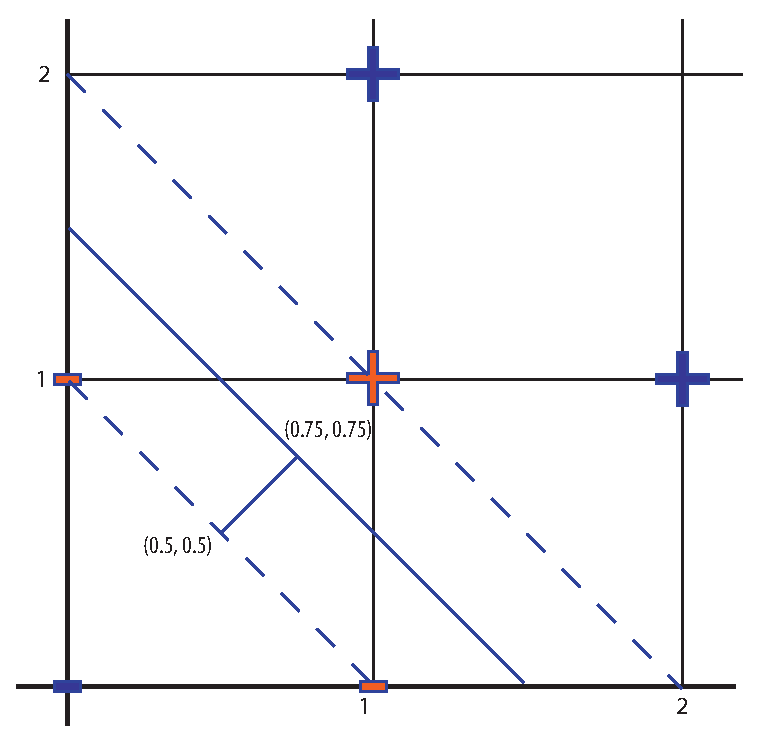
\includegraphics[scale=1]{supportvectors.eps}
\caption{Support vectors, margins, and the optimal separating line.}
\label{fig:vector}
\end{center}
\end{figure}



\item \textbf{2-norm soft margin: }
\begin{enumerate}
\item %a
\begin{align*}
L(\vec{w}, b, \vec{\xi},\vec{\alpha},\vec{\mu}) &= \frac{1}{2}\left(\vec{w} \cdot \vec{w}\right) + \frac{C}{2}\sum_i \xi_i^2 + \sum_i \alpha_i \left[ 1 - y_i \left( \vec{w}\cdot \vec{x_i}+b+\xi_i  \right) \right] - \sum_i \mu_i \xi_i
\end{align*}

\item %b
\begin{align*}
\frac{\partial L}{\partial w_j} &= w_j - \sum_i \alpha_i y_{i,j}\\
\frac{\partial L}{\partial \vec{w}} &= \vec{w} - \sum_i \alpha_i y_i \vec{x_i} \\
\vec{w} &= \sum_i \alpha_i y_i \vec{x_i} \\
\frac{\partial L }{\partial \xi_j} &= C\xi_j - \alpha_jy_j - \mu_j\\
\xi_j &= \frac{\alpha_j y_j + \mu_j}{C} \\
\frac{\partial L}{\partial b} &= \sum_i \alpha_i y_i \\
\sum_i \alpha_i y_i &= \vec{\alpha} \cdot \vec{y} = 0
\end{align*}

\item %c
\begin{align*}
L_{\text{sub}}\left(\vec{\alpha},\vec{\mu}\right) &=
\frac{1}{2}\left( \sum_i \alpha_i y_i \vec{x_i}\right) 
\left( \sum_i \alpha_i y_i \vec{x_i} \right) \\
&+ \frac{C}{2} \sum_i \left( \frac{\alpha_i y_i + \mu_i }{C} \right)^2 \\
&+ \sum_i \alpha_i \left[ 1-y_i \left( \vec{x_i} \left( \sum_j \alpha_j y_j \vec{x_j}\right) + b + \frac{\alpha_i y_i +\mu_i}{C} \right) \right] \\
&- \sum_i \mu_i \left(\frac{\alpha_i y_i + \mu_i}{C}\right) \\
L_{\text{sub}}\left(\vec{\alpha},\vec{\mu}\right) &= \frac{1}{2} \sum_{i,j}\alpha_i \alpha_j y_i y_j \vec{x_i}\cdot \vec{x_j} \\
&+ \frac{1}{2C} \sum_i\left(\alpha_i y_i +\mu_i\right)^2 \\
&+ \sum_i \alpha_i - \sum_{i,j} \alpha_i \alpha_j y_i y_j \left( \vec{x_i} \cdot \vec{x_j}\right) \\
&- \frac{1}{C}\sum_i \alpha_i y_i \left( \alpha_i y_i - \mu_i\right) \\
&- \frac{1}{C}\sum_i \mu_i \left( \alpha_i y_i - \mu_i\right) \\
L_{\text{sub}}\left(\vec{\alpha},\vec{\mu}\right) &= \frac{-1}{2}\sum_{i,j} \alpha_i \alpha_j y_i y_j \left(\vec{x_i} \cdot \vec{x_j}\right) \\
&+ \frac{1}{2C} \sum_i\left(\alpha_i y_i + \mu_i \right)^2 + \sum_i \alpha_i \\
&- \frac{1}{C} \sum_i \alpha_i y_i \left(\alpha_i y_i +\mu_i \right) \\
&- \frac{1}{C} \sum_i \mu_i \left( \alpha_i y_i + \mu_i \right) \\
L_{\text{sub}}\left(\vec{\alpha},\vec{\mu}\right) &= \sum_i \alpha_i - \frac{1}{2} \sum_{i,j} \alpha_i \alpha_j y_i y_j \left( \vec{x_i} \cdot \vec{x_j} \right) \\
&+ \frac{1}{C} \sum_i \left[ \frac{1}{2}\left(\alpha_i y_i + \mu_i \right)^2 - \left( \alpha_i y_i + \mu_i \right)^2\right] \\
L_{\text{sub}}\left(\vec{\alpha},\vec{\mu}\right) &= \sum_i \alpha_i - \frac{1}{2} \sum_{i,j}\alpha_i \alpha_j y_i y_j\left(\vec{x_i}\cdot \vec{x_j}\right) - \frac{1}{2C} \sum_i \left(\alpha_i y_i + \mu_i\right)^2
\end{align*}


\item %d
The equation for $L_{\text{sub}}\left(\vec{\alpha},\vec{\mu}\right)$ differs from $L_{\text{sub}_1}\left(\vec{\alpha}\right)$ only by the $- \frac{1}{2C} \sum_i \left(\alpha_i y_i + \mu_i\right)^2$ term. This term is always going to be negative which tells us that $L_{\text{sub}}\left(\vec{\alpha},\vec{\mu}\right) \leq L_{\text{sub}_1}\left(\vec{\alpha}\right) \forall \vec{\alpha},\vec{\mu} \in \Re^n \Rightarrow \text{max}_{\alpha,\mu} L_{\text{sub}}\left(\vec{\alpha},\vec{\mu}\right) \leq \text{max}_\alpha L_{\text{sub}_1}\left(\vec{\alpha}\right)$. The new function is still constrained by $\alpha,\mu \geq 0$.

We can also calculate $\frac{\partial L_{\text{sub}}\left(\vec{\alpha},\vec{\mu}\right)}{\partial \mu_k}$ and use that to get an intuition for what will change with the function. 
\begin{align*}
\frac{\partial L_{\text{sub}}\left(\vec{\alpha},\vec{\mu}\right)}{\partial \mu_k} &= \frac{-1}{2C} \left( 2 \alpha_k y_k + 2 \mu_k \right) \\
&= \frac{\alpha_k y_k + \mu_k}{C}\\
\mu^*_k &= -\alpha_k y_k \\
y_k < 0 &\Rightarrow \mu_k = \alpha_k \\
y_k \geq 0 &\Rightarrow \mu_k = 0 \\
\text{max}_{\mu} L_{\text{sub}}\left(\vec{\alpha},\vec{\mu}\right) &= L_{\text{sub}_1}\left(\vec{\alpha}\right) - \frac{1}{2C}\sum_{i: y_i = 1} \alpha_i^2 
\end{align*}

The above equation for maximizing $\mu$ tells us that maximizing $\alpha$ will be very similar to before, but perhaps less than before if there are lots of positive examples.

\end{enumerate}
\end{enumerate}
\end{document}
